\section{Plataforma de Evaluación}

\vspace{0.5cm}

\Large\scshape
\begin{center}
    Análisis de la plataforma de evaluación de celdas de combustible
\end{center}
\normalfont

\divider

En este capítulo, se realiza un detallado análisis de la Plataforma Experimental de Evaluación de Módulos de Celdas de Combustible de la figura \ref{diag_plataforma}, la cuál consiste en cuatro subsistemas o bloques distintos: 

\begin{itemize}
    \item Emulador de Celdas de Combustible
    \item Conversor CC-CC Conmutado
    \item Sistema de Control
    \item Carga Electrónica Variable
\end{itemize}

\begin{figure}[h]
    \centering
    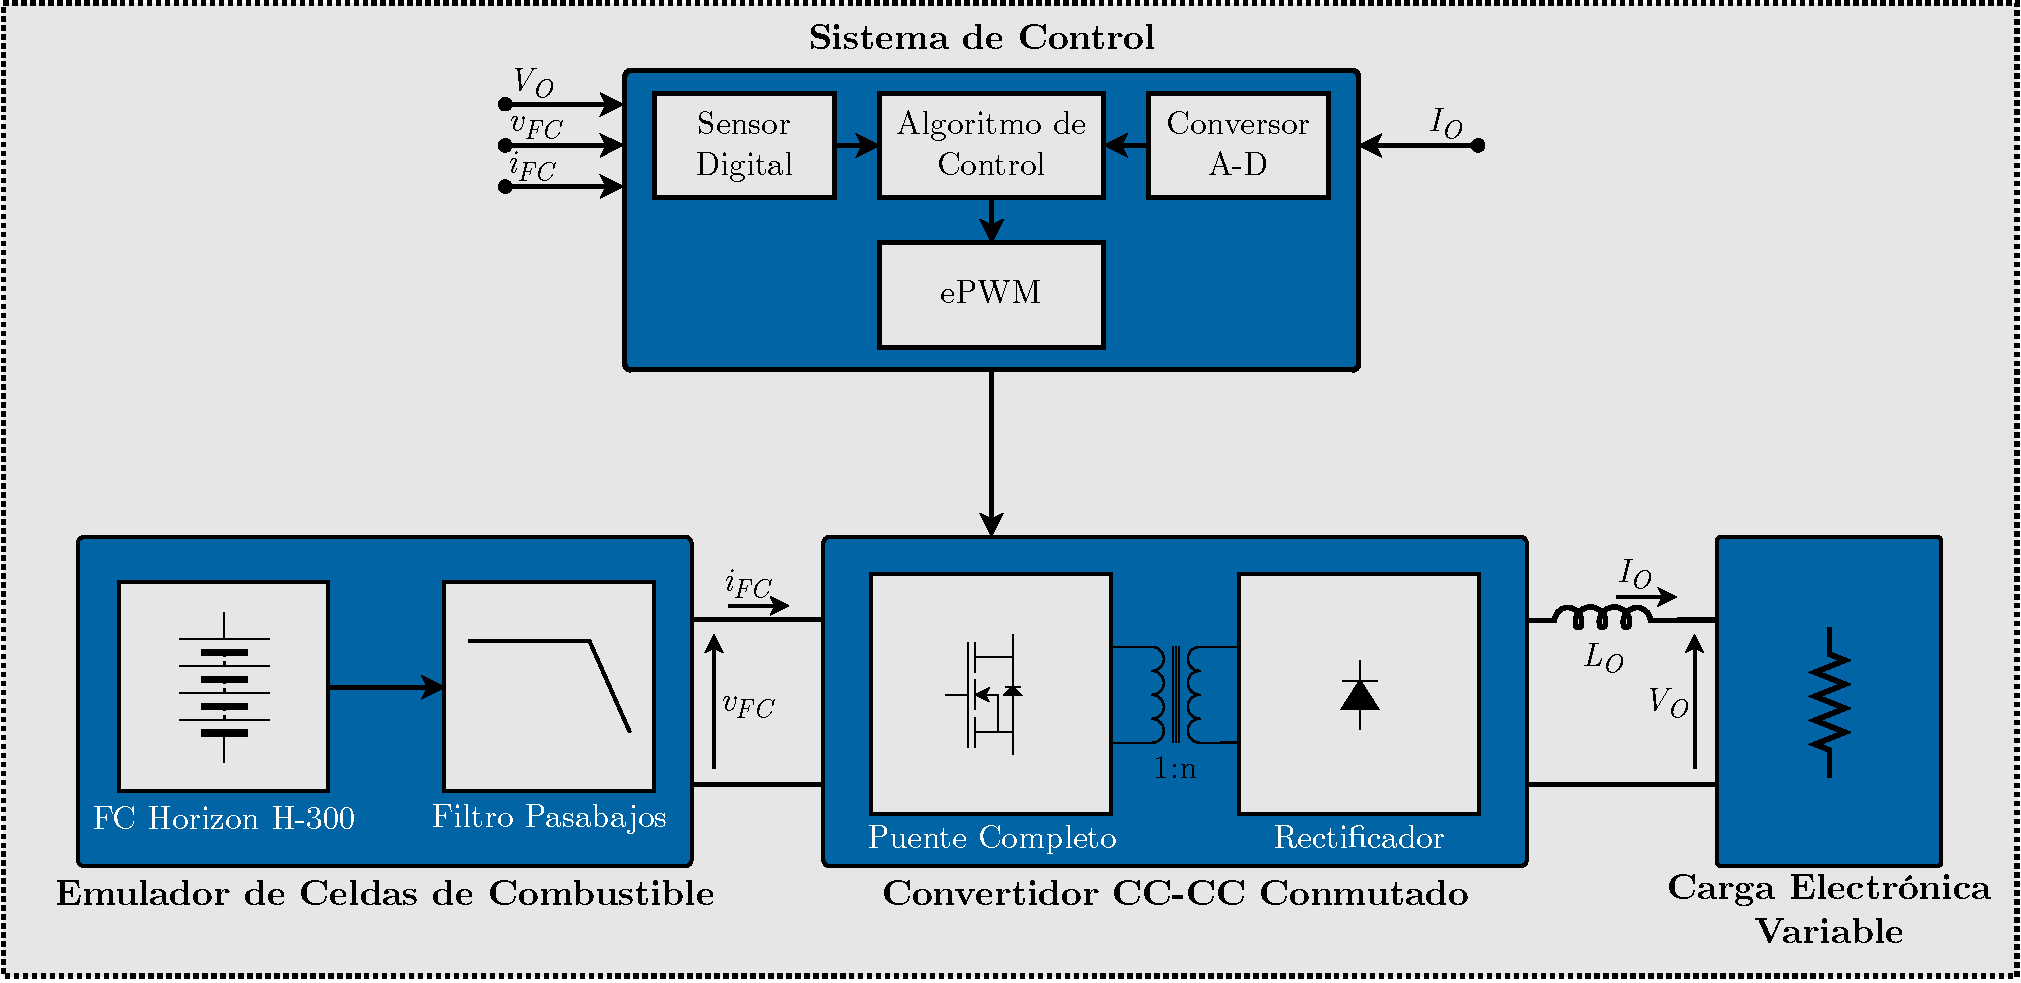
\includegraphics[scale=0.4]{Imagenes/Plataforma Experimental.pdf}
    \caption{Diagrama de la plataforma experimental de evaluación, con sus cuatro bloques principales.}
    \label{diag_plataforma}
\end{figure}

Esta plataforma, con sus distintos bloques, se encarga de evaluar la \textit{performance} de celdas de combustible conectadas a un sistema híbrido de generación. Con este fin, un emulador de celdas de combustible toma el puesto de celdas de combustible reales, y una carga electrónica variable se utiliza para simular cualquier tipo de condiciones de carga que se deseen en el bus de CC. Para poder conectar el emulador a la carga, se debe implementar un subsistema (Conversor CC-CC Conmutado) que adapte los niveles de tensión de salida del emulador de celdas a la tensión fija de salida en la carga, adicionando un módulo de control que monitorea los estados del conversor, y los controla mediante los disparos de las llaves del puente completo.\\

El principal objetivo de este proyecto es el diseño e implementación de la etapa de adaptación de tensión (es decir, el conversor con su sistema de control), pero se hace un estudio detallado de todas los componentes de la plataforma, de manera de obtener un entendimiento más completo de todo el sistema. Por esta razón, a continuación se hace un análisis en profundidad de cada una de las partes individuales, comenzando por el emulador de celdas de combustible.\\

\subsection{Emulador de Celdas de Combustible}

A pesar de que las celdas de combustible son una tecnología de hace más de un siglo y medio (desarrollada por primera vez por el físico galés Sir William Grove en 1842), hoy en día despiertan un particular interés en el campo de la generación renovable por su alta eficiencia, su dependencia en recursos obtenibles fácilmente de maneras ambientalmente amigables, y por la generación de agua como único deshecho.\\

Por estas razones se eligió trabajar con esta tecnología, particularmente con el tipo de celda más común hoy en día, las Celdas de Combustible de Membrana de Intercambio Protónico o PEM-FC (del inglés \textit{Proton Exchange Membrane Fuel Cell}), cuyo funcionamiento se profundiza más adelante.\\

\subsubsection{Principio de Funcionamiento de las Celdas de Combustible}

Esencialmente, una celda de combustible es una celda galvánica o celda voltáica en la cual la energía libre de una reacción química redox (entre un combustible y un agente oxidante) se convierte a energía eléctrica mediante una corriente y una diferencia de potencial$^{[FC-FundamentalsAndApplications]}$. En nuestro caso particular, el combustible es el hidrógeno molecular ($H_2$), el agente oxidante es el oxígeno ($O_2$) abundante en la atmósfera, y los productos son la energía eléctrica y el agua ($H_2O$) según indica la siguiente ecuación química balanceada.

\begin{equation}\label{redox_celda}
    2H_2\ +\ O_2\ \longrightarrow\ 2H_2O
\end{equation}

La estructura interna de una celda de combustible, visible en la figura \ref{fuel_cell}, consiste de un ánodo (electrodo negativo) al cual ingresan las moléculas de hidrógeno, un cátodo (electrodo positivo) en el que ingresa el oxígeno y se despide el agua, y un electrolito como como interfaz entre ánodo y cátodo. La carga es conectada entre el ánodo y el cátodo.

\begin{figure}[h]
    \centering
    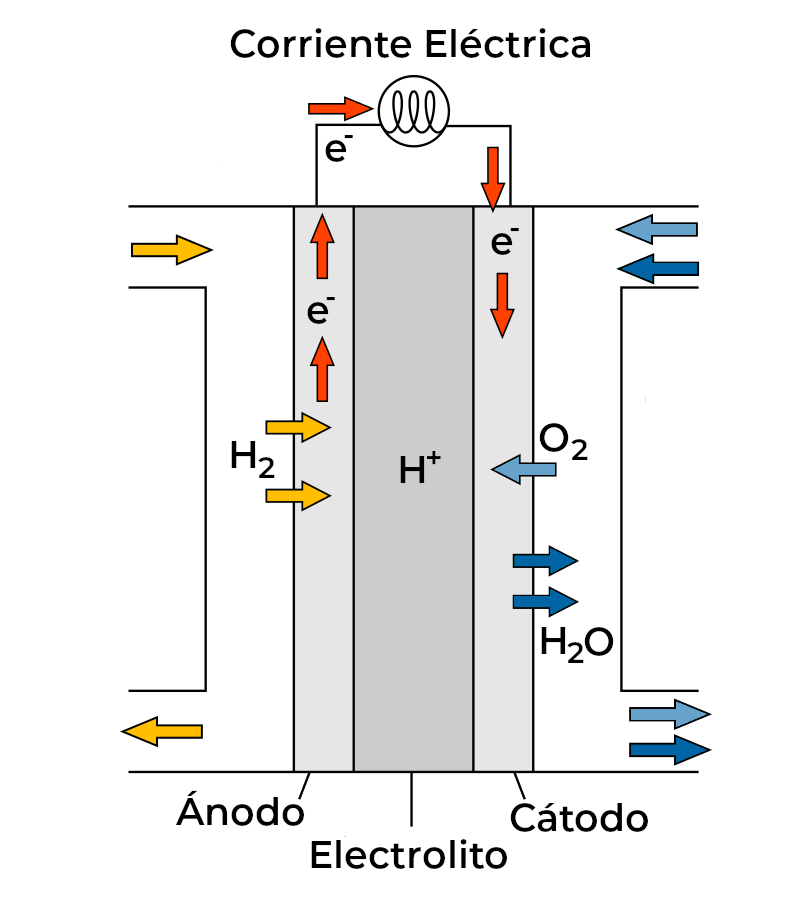
\includegraphics[scale=0.35]{Imagenes/Fuel Cell.png}
    \caption{Esquema de una celda de combustible, con todos sus componentes indicados (Placeholder).}
    \label{fuel_cell}
\end{figure}

La reacción redox de la ecuación \ref{redox_celda}, dentro de una celda de combustible como la del esquema, en realidad se separa en dos reacciones parciales distintas:

\begin{equation}\label{redox_anodo}
    2H_2\ \longrightarrow\ 4H^{+}\ +\ 4e^-
\end{equation}

\begin{equation}\label{redox_catodo}
    4H^{+}\ +\ 4e^-\ +\ O_2\longrightarrow\ 2H_2O
\end{equation}

De esta manera, alimentado simultáneamente el terminal negativo con combustible (hidrógeno) y el terminal positivo con oxidante (oxígeno) se producen las dos reacciones en las superficies de contacto del electrolito:

\begin{itemize}
    \item \textbf{En el ánodo} las moléculas de $H_2$ pierden sus electrones, bifurcándose los iones positivos de hidrógeno ($H^{+}$) por el electrolito y los electrones libres a través de la carga (ecuación \ref{redox_anodo}). Es una reacción exotérmica (libera calor) que resulta en el calentamiento de la celda.
    \item \textbf{En el cátodo} los iones $H^{+}$ del electrolito, los electrones libres, y las moléculas de oxígeno reaccionan para formar como producto el agua (ecuación \ref{redox_catodo}).
\end{itemize}

Mediante este proceso electroquímico se generan dos corrientes distintas: una corriente interna de iones $H^{+}$ (cargas positivas) en el electrolito, desde el ánodo hacia el cátodo; y una corriente externa de electrones $e^-$ (cargas negativas) circulando por la carga, en el mismo sentido que la corriente de iones. Esta última corriente de electrones es la que nos resulta útil para poder alimentar algún tipo de carga.\\

\subsubsection{Aspectos Constructivos de una Celda}



\subsubsection{De Celda a Pila de Combustible}

Sin embargo, una celda de combustible individual como en la figura \ref{fuel_cell} no es capaz de entregar una diferencia de potencial lo suficientemente alta para la gran mayoría de las aplicaciones, con una tensión de celda común situada entre 0.7 V y 1.3 V, dependiendo de varios aspectos constructivos específicos de la celda.\\